\documentclass[12pt,a4paper]{article}
\usepackage[utf8]{inputenc}
\usepackage{mathptmx} % Times New Roman
\usepackage[margin=2cm]{geometry}
\usepackage{titlesec}
\usepackage{indentfirst}
\usepackage{setspace}
\usepackage{graphicx}
\usepackage{caption}
\usepackage{longtable}
\usepackage{booktabs}
\usepackage{url}
\usepackage[hidelinks]{hyperref}
\usepackage{calc}
\usepackage{array}
\usepackage{soul}
\usepackage{amsmath}

\titleformat{\section}{\fontsize{14pt}{16.8pt}\selectfont\bfseries}{\thesection}{1em}{}
\titlespacing*{\section}{0pt}{14pt}{0pt}

\titleformat{\subsection}{\fontsize{12pt}{14.4pt}\selectfont\bfseries}{\thesubsection}{1em}{}
\titlespacing*{\subsection}{0pt}{12pt}{0pt}

\titleformat{\subsubsection}{\fontsize{12pt}{14.4pt}\selectfont\itshape}{\thesubsubsection}{1em}{}
\titlespacing*{\subsubsection}{0pt}{12pt}{0pt}

\setlength{\parindent}{0.5cm}
\setlength{\parskip}{6pt}
\setstretch{1.25} % Line spacing of at least 18pt

\pagestyle{plain} % Page numbers starting at 1, no headers

\begin{document}


\textbf{Full paper Template: Author Guidelines}

First Author\textsuperscript{1}, Second Author \textsuperscript{2},
Third Author \textsuperscript{2}*

\begin{quote}
\textsuperscript{1} Department/Unit (if applicable), Organization, City,
Brazil, author1@email.com.br*

\textsuperscript{2} Department/Unit (if applicable), Organization, City,
Brazil, \{author2, author3\}@email.com.br *

*Those information should be filled only after the work has been
approved
\end{quote}

\textbf{Abstract}

\emph{The abstract must be limited to 200-400 words. Use Times New
Roman, 12pt, italics, with line spacing of 1,5. Indent the first line of
the paragraph with 0.5cm. Justify the text in a paragraph on the left-
and right-hand side. The abstract should briefly describe the research
problem, the approach or methodology, and explicitly highlight the main
contribution and key findings of the work. Abstracts that do not clearly
state the main contribution and results of the paper may not be
considered for review. Separate sections with a single line.}

\textbf{Keywords:} Include 3 to 5 keywords, separated by ``;''; using
lower case (except names), and Times New Roman 12. At least one of them
must be selected from the following core areas: Cadastre, Cartography,
Geodesy, Photogrammetry or Remote Sensing.

\section{Introduction}

The XIV Brazilian Colloquium on Geodetic Sciences (CBCG) is an event
promoted by the Graduate Program in Geodetic Sciences (PPGCG), linked to
the Department of Geomatics within the Sector of Earth Sciences at the
Federal University of Paraná (UFPR). Since its inception in 1999,
colloquium has established itself as a vital space for meeting,
dialogue, and the dissemination of scientific, technological, and
innovative knowledge in the field of Geodetic Sciences.

Throughout its previous editions, the CBCG has met the demand for
academic and scientific events focused on Geodesy, Cartography, and
Remote Sensing, bringing together researchers, professionals, faculty,
and students from various regions of Brazil and abroad. In its
fourteenth edition, the event reaffirms its commitment to the exchange
of ideas and the strengthening of the scientific community.

This document provides formatting instructions for authors preparing
full-length research papers for the XIV CBCG. Authors are requested to
strictly follow these guidelines. The present MS Word document may be
used as a template.

Submitted papers must be original and must not have been previously
published, nor be under consideration for publication elsewhere.
References should be comprehensive and must adequately cover relevant
prior research in the field.

Please consider that the manuscript must clearly include: the problem or
research question, the methodology or approach, the main contribution of
the paper, and the principal results or implications.

\section{Manuscript Submission}

Manuscripts must be submitted electronically as a \emph{Portable
Document Format} (.PDF format) via the event website
(https://cbcg.ufpr.br). The manuscript must not exceed twelve pages, and
the file size must be limited to 6 MB, including figures, tables,
references, and appendices. Each paper will be reviewed by at least two
anonymous reviewers. Their evaluations will be used to determine
acceptance and, when applicable, will be forwarded to the author(s) with
suggested revisions.

Once the manuscript has been accepted, a final version (page proof) in
PDF format will be sent to the author(s) for approval prior to
publication. To avoid delays in the publication process, authors are
strongly encouraged to follow the style guidelines carefully.

\textbf{Note}: To ensure a double-blind review process, authors must
remove all identifying information from the initial submission. This
includes author names and affiliations (typically listed below the
title), as well as any identifying information in the document
properties. After the review process and any required revisions, authors
should restore this information in the final version.

\section{Copyright and Disclosure}

\subsection{Copyright}

By submitting a paper to this event, authors agree to the following
terms:

\begin{enumerate}
\def\labelenumi{\alph{enumi}.}
\item
  Authors retain copyright of their work while granting the event the
  right to publish and make it available on its website under a Creative
  Commons Attribution License. This license allows others to access,
  use, and share the work, provided that proper acknowledgment is given
  to the original authors and to its initial publication in the event.
\item
  Authors are encouraged to post and share their work online (e.g., in
  institutional repositories or personal websites) at any time after
  publication on the event website.
\end{enumerate}

\subsection{Disclosure}

If the submission requires approval by an institution, company, or
government agency prior to publication, the author(s) must ensure that
such permission has been obtained in writing, confirming that the
information contained in the paper may be made publicly available on the
event website.

Author(s) and/or their organizations retain the right to reuse the work,
in whole or in part. The event organizers do not control the commercial
use of published material. However, it is assumed that all submissions
have been properly authorized and that the author(s) have the necessary
rights to disclose the information contained therein.

\subsection{\texorpdfstring{Paper Formatting Guidelines (Times New
Roman, 14pt, bold)
}{Paper Formatting Guidelines (Times New Roman, 14pt, bold) }}

\subsubsection{General (Times New Roman, 12pt, Bold)}

The table below summarizes the most important aspects of the desired
layout of the paper.

Table 1. Formatting summary

\begin{longtable}[]{@{}
  >{\raggedright\arraybackslash}p{(\columnwidth - 2\tabcolsep) * \real{0.2370}}
  >{\raggedright\arraybackslash}p{(\columnwidth - 2\tabcolsep) * \real{0.7630}}@{}}
\toprule\noalign{}
\begin{minipage}[b]{\linewidth}\raggedright
\textbf{Item}
\end{minipage} & \begin{minipage}[b]{\linewidth}\raggedright
\textbf{Description}
\end{minipage} \\
\midrule\noalign{}
\endhead
\bottomrule\noalign{}
\endlastfoot
\begin{minipage}[t]{\linewidth}\raggedright
\begin{quote}
Page size \& margins
\end{quote}
\end{minipage} & \begin{minipage}[t]{\linewidth}\raggedright
\begin{quote}
A4 Portrait; all margins 2cm
\end{quote}
\end{minipage} \\
\begin{minipage}[t]{\linewidth}\raggedright
\begin{quote}
Page numbers
\end{quote}
\end{minipage} & \begin{minipage}[t]{\linewidth}\raggedright
\begin{quote}
Yes, starting at 1
\end{quote}
\end{minipage} \\
\begin{minipage}[t]{\linewidth}\raggedright
\begin{quote}
Footer / Headers
\end{quote}
\end{minipage} & \begin{minipage}[t]{\linewidth}\raggedright
\begin{quote}
None (NB: footnotes are \emph{not} permitted)
\end{quote}
\end{minipage} \\
\begin{minipage}[t]{\linewidth}\raggedright
\begin{quote}
Title
\end{quote}
\end{minipage} & \begin{minipage}[t]{\linewidth}\raggedright
\begin{quote}
Times New Roman, 16pt, bold, first letter in capitals, centered,
followed by a single blank line, 12pt.
\end{quote}
\end{minipage} \\
\begin{minipage}[t]{\linewidth}\raggedright
\begin{quote}
Author and co-authors
\end{quote}
\end{minipage} & \begin{minipage}[t]{\linewidth}\raggedright
\begin{quote}
Times New Roman, 12pt, centered - author and co-author names in one
line, followed by a single blank line, 12pt.
\end{quote}
\end{minipage} \\
\begin{minipage}[t]{\linewidth}\raggedright
\begin{quote}
Author affiliations
\end{quote}
\end{minipage} & \begin{minipage}[t]{\linewidth}\raggedright
\begin{quote}
Times New Roman, 12pt, centered -- each author's full affiliation (i.e.
company / organization), full contact details of the corresponding
author only, followed by a single blank line, 12pt.
\end{quote}
\end{minipage} \\
\begin{minipage}[t]{\linewidth}\raggedright
\begin{quote}
Key-words
\end{quote}
\end{minipage} & \begin{minipage}[t]{\linewidth}\raggedright
\begin{quote}
Times New Roman, 12pt, left-justified, separated by semicolon, followed
by a single blank line,12pt.
\end{quote}
\end{minipage} \\
\begin{minipage}[t]{\linewidth}\raggedright
\begin{quote}
Abstract
\end{quote}
\end{minipage} & \begin{minipage}[t]{\linewidth}\raggedright
\begin{quote}
Times New Roman, 12pt, Italics, with line spacing of 1,5. Indent the
first line of the paragraph with 0.5cm. Justify the text in a paragraph
on the left- and right-hand side.

Separate sections with a single line. 200 - 400 words
\end{quote}
\end{minipage} \\
\begin{minipage}[t]{\linewidth}\raggedright
\begin{quote}
Headings
\end{quote}
\end{minipage} & \begin{minipage}[t]{\linewidth}\raggedright
\begin{quote}
Times New Roman, 14pt, bold, left-justified, first letter in capitals,
one blank line above.
\end{quote}
\end{minipage} \\
\begin{minipage}[t]{\linewidth}\raggedright
\begin{quote}
Sub-headings
\end{quote}
\end{minipage} & \begin{minipage}[t]{\linewidth}\raggedright
\begin{quote}
Times New Roman, 12pt, bold, left-justified, in proper case, one blank
line above.
\end{quote}
\end{minipage} \\
\begin{minipage}[t]{\linewidth}\raggedright
\begin{quote}
Sub-sub-headings
\end{quote}
\end{minipage} & \begin{minipage}[t]{\linewidth}\raggedright
\begin{quote}
Times New Roman, 12pt, italic, left-justified, in proper case, one blank
line above.
\end{quote}
\end{minipage} \\
\begin{minipage}[t]{\linewidth}\raggedright
\begin{quote}
Heading numbering
\end{quote}
\end{minipage} & \begin{minipage}[t]{\linewidth}\raggedright
\begin{quote}
Use the decimal system of heading numbering, with no more than three
levels.
\end{quote}
\end{minipage} \\
\end{longtable}

Source: Author and year (if necessary)

\subsubsection{Body Text}

Body Text should be Times New Roman, 12pt, with line spacing of at least
18pt. Indent the first line of the paragraph with 0.5cm. Justify the
text in a paragraph on the left- and right-hand side. Use a spacing of
6pt before each paragraph.

\subsubsection{Symbols and units}

SI units should be used. Where abbreviations for units are used, there
should be space between the value and the unit - i.e., `10 km', not
`10km' -- and angles should be `25°30\textquotesingle S', not `25°
30\textquotesingle{} S'. Use italics for Greek or Roman text or
abbreviations (\emph{e.g., et al.}).

\subsubsection{Equations}

Equations should be numbered consecutively throughout the text with
Arabic numerals in parentheses (not brackets), right-justified, as in
(1). When referring to an equation in the text, use "Equation (1)" or
"Eq. (1)". The equation should be indented by 7,5cm, with the equation
number right justified. Equation Editor (MSWord97-2003) or MathType
should be used to create the equations. Either plain or italics style
may be used for the variables, as long as there is consistency in style.
Use boldface for vectors and matrices.

\(N = \ \gamma + \frac{\overline{\alpha}}{\sum_{i = 1}^{n}b_{i}}\) (1)

\subsubsection{Figures, photographs and illustrations}

Figures should be provided in a standard format (e.g. jpeg, tiff, bmp)
and should be of high resolution (450dpi). Figures shall be numbered
consecutively with a brief caption, which should be in Times New Roman,
12pt, above the figure, centered, and not bold, the source/authorship of
the figure should be in Times New Roman, 12pt, below the figure,
centered, and not bold. The figure, photograph or illustration should
also be centered. Authors are encouraged to make use of color in all
graphics, figures and photographs. The figure should be in the document,
as close as practicable to the first reference to it. Refer to the
example below.

Figure 1. South African Geoid Model 2010

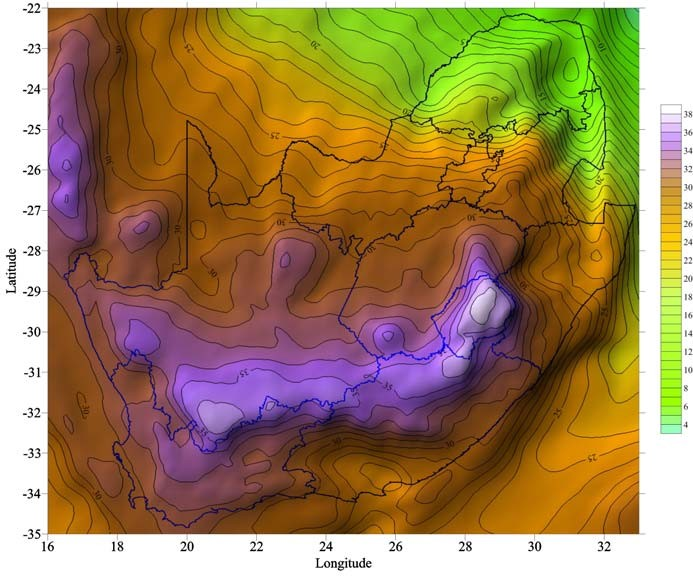
\includegraphics[width=4.62325in,height=3.86in]{media/media/image1.jpg}

Source: Author and year (if necessary)

\subsubsection{Tables}

Tables should be numbered consecutively and should have captions. The
table caption should be in Times New Roman, 12pt, positioned above the
table, centered, and not in bold. Text inside the table should
preferably be Times New Roman, 10pt, centered, with the headings in
bold, the source/authorship of the table should be in Times New Roman,
12pt, below the table, centered, and not bold. Each table shall be in
the document as close as practicable to the first reference to it. Refer
to the example below.

Table 2. Differences with GPS/Levelling - Western Cape Province

\begin{longtable}[]{@{}
  >{\raggedright\arraybackslash}p{(\columnwidth - 8\tabcolsep) * \real{0.1993}}
  >{\raggedright\arraybackslash}p{(\columnwidth - 8\tabcolsep) * \real{0.2033}}
  >{\raggedright\arraybackslash}p{(\columnwidth - 8\tabcolsep) * \real{0.2203}}
  >{\raggedright\arraybackslash}p{(\columnwidth - 8\tabcolsep) * \real{0.1945}}
  >{\raggedright\arraybackslash}p{(\columnwidth - 8\tabcolsep) * \real{0.1826}}@{}}
\toprule\noalign{}
\begin{minipage}[b]{\linewidth}\raggedright
\textbf{Model}
\end{minipage} & \begin{minipage}[b]{\linewidth}\raggedright
\textbf{Min. (cm)}
\end{minipage} & \begin{minipage}[b]{\linewidth}\raggedright
\textbf{Max. (cm)}
\end{minipage} & \begin{minipage}[b]{\linewidth}\raggedright
\textbf{Mean (cm)}
\end{minipage} & \begin{minipage}[b]{\linewidth}\raggedright
\textbf{Std. Dev. (cm)}
\end{minipage} \\
\midrule\noalign{}
\endhead
\bottomrule\noalign{}
\endlastfoot
AGP2003 & - 76 & - 38 & - 63 & 9 \\
EGM96 & - 97 & - 62 & - 55 & 20 \\
\end{longtable}

Source: Author and year (if necessary)

\subsubsection{References}

In-text citations must use numerical identifiers enclosed in brackets,
such as {[}1{]}. The reference list at the end of the document must be
organized in alphabetical order by the first author\textquotesingle s
last name and numbered accordingly, ensuring a direct correlation
between the in-text citations and the final list. \textbf{Please note
that in-text citation numbers correspond strictly to the
item\textquotesingle s position in the alphabetical reference list, and
not to their order of appearance in the text.} For references, use Times
New Roman, 11pt, first line hanging by 0.5cm. Use a line spacing of at
least 15pt. Use the ABNT style for reference. References should be
listed in alphabetical order and presented as shown in the examples at
the end of this document. References should follow one another, with no
blank lines in between.

\textbf{Book}

Author, \emph{Book Title}, Edition, Place of Publication, Publisher,
Year. Example:

Czinkota, M. R.; Ronkainen, A. I. \emph{International marketing}. 7. ed.
Mason, Ohio: Thomson/South-Western, 2004.

\textbf{Chapter in Book}

Author, `Chapter title', in Editors (eds.), \emph{Book Title}, Place of
publication, Publisher, Year. Example:

North, D. `Energy use at home'. In: Scott, S.; Peel, N. (org.).
\emph{Energy conservation}. London: Academic Press, 1980.

\textbf{Full-text journal article}

Author, `Article title', \emph{Journal Title}, Volume (Issue), Pages,
Year. Example:

Rasid, Z. M.; Parish, T. S., `The effects of two types of relaxation
training on students\textquotesingle{} levels of anxiety',
\emph{Adolescence}, 33(129), 99--110, 1998.

\textbf{Conference Proceedings}

Author Year, \emph{Article title}, in Editors (eds.), \emph{Proceedings
Title}, Place and date of conference, Place of publication, Publisher,
Date of publication, Pages. Example:

Merry, C. L. Recent variations in mean sea level. In: Sünkel, H.; Baker,
T. (org.). \emph{Sea Surface Topography and the Geoid}. Edinburgh, July
1989. New York: Springer-Verlag, 1990. p. 149-157.

\textbf{Journal article on the WWW}

Author Year, \emph{Article title}, \emph{Journal Title}, Volume (Issue),
Available at: URL, Accessed Day Month Year. Example:

Griffith, A. I. Coordinating family and school: mothering for schooling.
\emph{Education Policy Analysis Archives}, v. 3, n. 1, 1995. Available
at:
\href{http://olam.ed.asu.edu/epaa/}{\ul{http://olam.ed.asu.edu/epaa/}}.
Accessed: 12 feb. 1997.

\textbf{Web document}

Author Year, \emph{Document title}, Place, Institution/Publisher,
Available at: URL, Accessed Day Month Year. Example:

Anderson, J. CASA approves Avgas Contamination Test. Canberra:
Department of Transport and Regional Services, 2000. Available at:
\href{http://www.dotrs.gov.au/media/anders/archive/2000/jan_00/al6_2000.htm}{\ul{http://www.dotrs.gov.au/media/anders/archive/2000/jan\_00/al6\_2000.htm}}.
Accessed: 7 feb. 2000.

\textbf{Web document (no author)}

\emph{Document title,} Year, Institution/Publisher, Available at: URL,
Accessed Day Month Year. Example:

Educating \emph{America for the 21st century: developing a strategic
plan for educational leadership.} Columbia University, 1994. Available
at:
\href{http://ariel.adgrp.com/~ghb/trips/940717_ICT/policy/ILT/EdPlan.html}{\ul{http://ariel.adgrp.com/\textasciitilde ghb/trips/940717\_ICT/policy/ILT/EdPlan.html}}.
Accessed: 16 may 1995.

\textbf{Web document (no publication date)}

Author {[}s.d.{]}, \emph{Document title}, Place, Institution/Publisher,
Available at: URL, Accessed Day Month Year. Example:

Sherman, C. \emph{The invisible web}. UK: Free Pint Limited, {[}s.d.{]}.
Available at:
\href{http://www.freepint.co.uk/issues/080600.htm\#feature}{\ul{http://www.freepint.co.uk/issues/080600.htm\#feature}}.
Accessed: 27 nov. 2000.

\textbf{Web site}

Organization Year, \emph{Website title}, Place, Available at: URL,
Accessed Day Month Year. Example:

THE BODY SHOP AUSTRALIA. \emph{The Body Shop Australia}. Mulgrave,
Victoria, 2003. Available at:
\href{http://www.thebodyshop.com.au/}{\ul{http://www.thebodyshop.com.au/}}.
Accessed: 31 jan. 2003.

\emph{\textbf{May 1, 2026}}


\end{document}
